\documentclass[twoside]{book}

% Packages required by doxygen
\usepackage{fixltx2e}
\usepackage{calc}
\usepackage{doxygen}
\usepackage[export]{adjustbox} % also loads graphicx
\usepackage{graphicx}
\usepackage[utf8]{inputenc}
\usepackage{makeidx}
\usepackage{multicol}
\usepackage{multirow}
\PassOptionsToPackage{warn}{textcomp}
\usepackage{textcomp}
\usepackage[nointegrals]{wasysym}
\usepackage[table]{xcolor}

% Font selection
\usepackage[T1]{fontenc}
\usepackage[scaled=.90]{helvet}
\usepackage{courier}
\usepackage{amssymb}
\usepackage{sectsty}
\renewcommand{\familydefault}{\sfdefault}
\allsectionsfont{%
  \fontseries{bc}\selectfont%
  \color{darkgray}%
}
\renewcommand{\DoxyLabelFont}{%
  \fontseries{bc}\selectfont%
  \color{darkgray}%
}
\newcommand{\+}{\discretionary{\mbox{\scriptsize$\hookleftarrow$}}{}{}}

% Page & text layout
\usepackage{geometry}
\geometry{%
  a4paper,%
  top=2.5cm,%
  bottom=2.5cm,%
  left=2.5cm,%
  right=2.5cm%
}
\tolerance=750
\hfuzz=15pt
\hbadness=750
\setlength{\emergencystretch}{15pt}
\setlength{\parindent}{0cm}
\setlength{\parskip}{3ex plus 2ex minus 2ex}
\makeatletter
\renewcommand{\paragraph}{%
  \@startsection{paragraph}{4}{0ex}{-1.0ex}{1.0ex}{%
    \normalfont\normalsize\bfseries\SS@parafont%
  }%
}
\renewcommand{\subparagraph}{%
  \@startsection{subparagraph}{5}{0ex}{-1.0ex}{1.0ex}{%
    \normalfont\normalsize\bfseries\SS@subparafont%
  }%
}
\makeatother

% Headers & footers
\usepackage{fancyhdr}
\pagestyle{fancyplain}
\fancyhead[LE]{\fancyplain{}{\bfseries\thepage}}
\fancyhead[CE]{\fancyplain{}{}}
\fancyhead[RE]{\fancyplain{}{\bfseries\leftmark}}
\fancyhead[LO]{\fancyplain{}{\bfseries\rightmark}}
\fancyhead[CO]{\fancyplain{}{}}
\fancyhead[RO]{\fancyplain{}{\bfseries\thepage}}
\fancyfoot[LE]{\fancyplain{}{}}
\fancyfoot[CE]{\fancyplain{}{}}
\fancyfoot[RE]{\fancyplain{}{\bfseries\scriptsize Generated by Doxygen }}
\fancyfoot[LO]{\fancyplain{}{\bfseries\scriptsize Generated by Doxygen }}
\fancyfoot[CO]{\fancyplain{}{}}
\fancyfoot[RO]{\fancyplain{}{}}
\renewcommand{\footrulewidth}{0.4pt}
\renewcommand{\chaptermark}[1]{%
  \markboth{#1}{}%
}
\renewcommand{\sectionmark}[1]{%
  \markright{\thesection\ #1}%
}

% Indices & bibliography
\usepackage{natbib}
\usepackage[titles]{tocloft}
\setcounter{tocdepth}{3}
\setcounter{secnumdepth}{5}
\makeindex

% Hyperlinks (required, but should be loaded last)
\usepackage{ifpdf}
\ifpdf
  \usepackage[pdftex,pagebackref=true]{hyperref}
\else
  \usepackage[ps2pdf,pagebackref=true]{hyperref}
\fi
\hypersetup{%
  colorlinks=true,%
  linkcolor=blue,%
  citecolor=blue,%
  unicode%
}

% Custom commands
\newcommand{\clearemptydoublepage}{%
  \newpage{\pagestyle{empty}\cleardoublepage}%
}

\usepackage{caption}
\captionsetup{labelsep=space,justification=centering,font={bf},singlelinecheck=off,skip=4pt,position=top}

%===== C O N T E N T S =====

\begin{document}

% Titlepage & ToC
\hypersetup{pageanchor=false,
             bookmarksnumbered=true,
             pdfencoding=unicode
            }
\pagenumbering{alph}
\begin{titlepage}
\vspace*{7cm}
\begin{center}%
{\Large My Project }\\
\vspace*{1cm}
{\large Generated by Doxygen 1.8.14}\\
\end{center}
\end{titlepage}
\clearemptydoublepage
\pagenumbering{roman}
\tableofcontents
\clearemptydoublepage
\pagenumbering{arabic}
\hypersetup{pageanchor=true}

%--- Begin generated contents ---
\chapter{Namespace Index}
\section{Namespace List}
Here is a list of all documented namespaces with brief descriptions\+:\begin{DoxyCompactList}
\item\contentsline{section}{\mbox{\hyperlink{namespace_smart}{Smart}} \\*Home-\/ino This is the dokumentation of the Source Code from the project \mbox{\hyperlink{namespace_smart}{Smart}} Home }{\pageref{namespace_smart}}{}
\end{DoxyCompactList}

\chapter{Hierarchical Index}
\section{Class Hierarchy}
This inheritance list is sorted roughly, but not completely, alphabetically\+:\begin{DoxyCompactList}
\item object\begin{DoxyCompactList}
\item \contentsline{section}{Python\+\_\+\+Client.\+Create\+Button}{\pageref{class_python___client_1_1_create_button}}{}
\item \contentsline{section}{Python\+\_\+\+Client.\+Create\+Label}{\pageref{class_python___client_1_1_create_label}}{}
\item \contentsline{section}{Python\+\_\+\+Client.\+Frame\+Buttons}{\pageref{class_python___client_1_1_frame_buttons}}{}
\item \contentsline{section}{Python\+\_\+\+Client.\+send\+Mail}{\pageref{class_python___client_1_1send_mail}}{}
\item \contentsline{section}{Python\+\_\+\+Client.\+Wifi\+Connect}{\pageref{class_python___client_1_1_wifi_connect}}{}
\item \contentsline{section}{Python\+\_\+\+Client.\+Window\+Function}{\pageref{class_python___client_1_1_window_function}}{}
\end{DoxyCompactList}
\end{DoxyCompactList}

\chapter{Class Index}
\section{Class List}
Here are the classes, structs, unions and interfaces with brief descriptions\+:\begin{DoxyCompactList}
\item\contentsline{section}{\mbox{\hyperlink{class_python___client_1_1_create_button}{Python\+\_\+\+Client.\+Create\+Button}} \\*This class creates default buttons }{\pageref{class_python___client_1_1_create_button}}{}
\item\contentsline{section}{\mbox{\hyperlink{class_python___client_1_1_create_label}{Python\+\_\+\+Client.\+Create\+Label}} \\*This class creates labels }{\pageref{class_python___client_1_1_create_label}}{}
\item\contentsline{section}{\mbox{\hyperlink{class_python___client_1_1_frame_buttons}{Python\+\_\+\+Client.\+Frame\+Buttons}} \\*This class handles the frame switch buttons }{\pageref{class_python___client_1_1_frame_buttons}}{}
\item\contentsline{section}{\mbox{\hyperlink{class_python___client_1_1send_mail}{Python\+\_\+\+Client.\+send\+Mail}} \\*Class to send emails }{\pageref{class_python___client_1_1send_mail}}{}
\item\contentsline{section}{\mbox{\hyperlink{class_python___client_1_1_wifi_connect}{Python\+\_\+\+Client.\+Wifi\+Connect}} \\*Class for the Wifi connection }{\pageref{class_python___client_1_1_wifi_connect}}{}
\item\contentsline{section}{\mbox{\hyperlink{class_python___client_1_1_window_function}{Python\+\_\+\+Client.\+Window\+Function}} \\*The class to setup the main tkinter window }{\pageref{class_python___client_1_1_window_function}}{}
\end{DoxyCompactList}

\chapter{Namespace Documentation}
\hypertarget{namespace_smart}{}\section{Smart Namespace Reference}
\label{namespace_smart}\index{Smart@{Smart}}


Home-\/ino This is the dokumentation of the Source Code from the project \mbox{\hyperlink{namespace_smart}{Smart}} Home.  




\subsection{Detailed Description}
Home-\/ino This is the dokumentation of the Source Code from the project \mbox{\hyperlink{namespace_smart}{Smart}} Home. 

\begin{DoxyAuthor}{Author}
Okan Dogtas \href{mailto:odogtas@uni-bremen.de}{\tt odogtas@uni-\/bremen.\+de} 
\end{DoxyAuthor}
\begin{DoxyDate}{Date}
2018-\/06-\/20
\end{DoxyDate}
\begin{DoxyCopyright}{Copyright}
G\+NU General Public License v3.\+0 
\end{DoxyCopyright}

\chapter{Class Documentation}
\hypertarget{class_python___client_1_1_create_button}{}\section{Python\+\_\+\+Client.\+Create\+Button Class Reference}
\label{class_python___client_1_1_create_button}\index{Python\+\_\+\+Client.\+Create\+Button@{Python\+\_\+\+Client.\+Create\+Button}}


This class creates default buttons.  


Inheritance diagram for Python\+\_\+\+Client.\+Create\+Button\+:\begin{figure}[H]
\begin{center}
\leavevmode
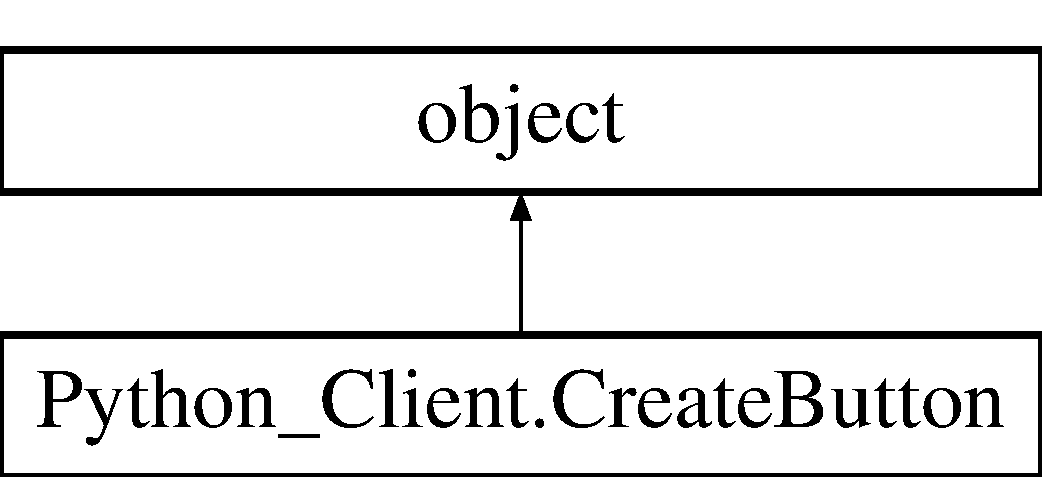
\includegraphics[height=2.000000cm]{class_python___client_1_1_create_button}
\end{center}
\end{figure}
\subsection*{Public Member Functions}
\begin{DoxyCompactItemize}
\item 
def \mbox{\hyperlink{class_python___client_1_1_create_button_ab0e1f7597f08c6abc36ebb034b228811}{\+\_\+\+\_\+init\+\_\+\+\_\+}} (self, parent, content, size, command)
\begin{DoxyCompactList}\small\item\em The default constructor. \end{DoxyCompactList}\end{DoxyCompactItemize}
\subsection*{Public Attributes}
\begin{DoxyCompactItemize}
\item 
\mbox{\Hypertarget{class_python___client_1_1_create_button_a78b040d7f0a668fc2c26ba8874cc2de6}\label{class_python___client_1_1_create_button_a78b040d7f0a668fc2c26ba8874cc2de6}} 
{\bfseries button}
\end{DoxyCompactItemize}


\subsection{Detailed Description}
This class creates default buttons. 

\subsection{Constructor \& Destructor Documentation}
\mbox{\Hypertarget{class_python___client_1_1_create_button_ab0e1f7597f08c6abc36ebb034b228811}\label{class_python___client_1_1_create_button_ab0e1f7597f08c6abc36ebb034b228811}} 
\index{Python\+\_\+\+Client\+::\+Create\+Button@{Python\+\_\+\+Client\+::\+Create\+Button}!\+\_\+\+\_\+init\+\_\+\+\_\+@{\+\_\+\+\_\+init\+\_\+\+\_\+}}
\index{\+\_\+\+\_\+init\+\_\+\+\_\+@{\+\_\+\+\_\+init\+\_\+\+\_\+}!Python\+\_\+\+Client\+::\+Create\+Button@{Python\+\_\+\+Client\+::\+Create\+Button}}
\subsubsection{\texorpdfstring{\+\_\+\+\_\+init\+\_\+\+\_\+()}{\_\_init\_\_()}}
{\footnotesize\ttfamily def Python\+\_\+\+Client.\+Create\+Button.\+\_\+\+\_\+init\+\_\+\+\_\+ (\begin{DoxyParamCaption}\item[{}]{self,  }\item[{}]{parent,  }\item[{}]{content,  }\item[{}]{size,  }\item[{}]{command }\end{DoxyParamCaption})}



The default constructor. 

in the instructor the button will be created with the given informations


\begin{DoxyParams}{Parameters}
{\em parent} & the parent frame / window of the button \\
\hline
{\em content} & the text, which will be written in the button \\
\hline
{\em size} & the font size of the button text \\
\hline
{\em command} & the executed command by pressing the button \\
\hline
\end{DoxyParams}


The documentation for this class was generated from the following file\+:\begin{DoxyCompactItemize}
\item 
Python\+\_\+\+Client.\+py\end{DoxyCompactItemize}

\hypertarget{class_python___client_1_1_create_label}{}\section{Python\+\_\+\+Client.\+Create\+Label Class Reference}
\label{class_python___client_1_1_create_label}\index{Python\+\_\+\+Client.\+Create\+Label@{Python\+\_\+\+Client.\+Create\+Label}}


This class creates labels.  


Inheritance diagram for Python\+\_\+\+Client.\+Create\+Label\+:\begin{figure}[H]
\begin{center}
\leavevmode
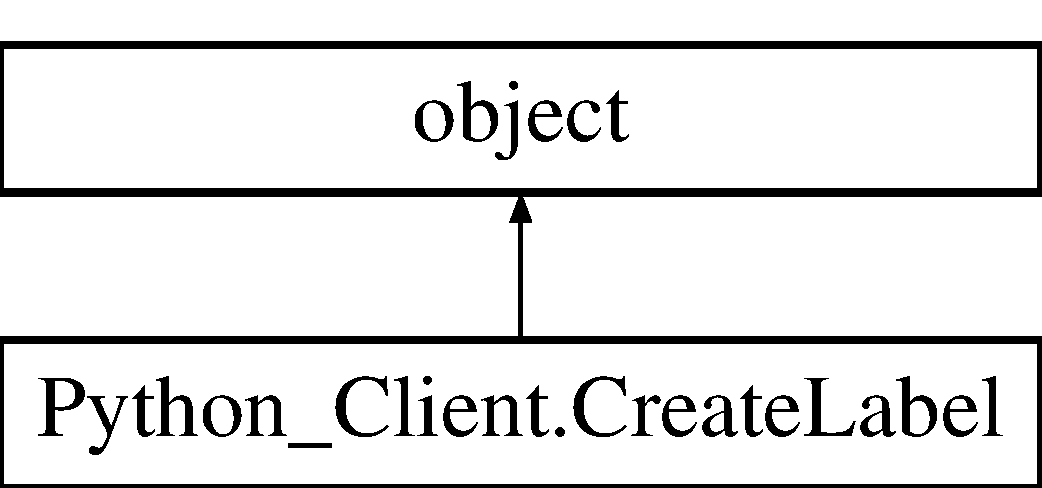
\includegraphics[height=2.000000cm]{class_python___client_1_1_create_label}
\end{center}
\end{figure}
\subsection*{Public Member Functions}
\begin{DoxyCompactItemize}
\item 
def \mbox{\hyperlink{class_python___client_1_1_create_label_a55df86d9d18bfc00d79dfb0e35fc1377}{\+\_\+\+\_\+init\+\_\+\+\_\+}} (self, parent, content, size, color)
\begin{DoxyCompactList}\small\item\em The default constructor. \end{DoxyCompactList}\end{DoxyCompactItemize}
\subsection*{Public Attributes}
\begin{DoxyCompactItemize}
\item 
\mbox{\Hypertarget{class_python___client_1_1_create_label_a39fd4147b815ba59bacf9d5d27ae9426}\label{class_python___client_1_1_create_label_a39fd4147b815ba59bacf9d5d27ae9426}} 
{\bfseries label}
\end{DoxyCompactItemize}


\subsection{Detailed Description}
This class creates labels. 

\subsection{Constructor \& Destructor Documentation}
\mbox{\Hypertarget{class_python___client_1_1_create_label_a55df86d9d18bfc00d79dfb0e35fc1377}\label{class_python___client_1_1_create_label_a55df86d9d18bfc00d79dfb0e35fc1377}} 
\index{Python\+\_\+\+Client\+::\+Create\+Label@{Python\+\_\+\+Client\+::\+Create\+Label}!\+\_\+\+\_\+init\+\_\+\+\_\+@{\+\_\+\+\_\+init\+\_\+\+\_\+}}
\index{\+\_\+\+\_\+init\+\_\+\+\_\+@{\+\_\+\+\_\+init\+\_\+\+\_\+}!Python\+\_\+\+Client\+::\+Create\+Label@{Python\+\_\+\+Client\+::\+Create\+Label}}
\subsubsection{\texorpdfstring{\+\_\+\+\_\+init\+\_\+\+\_\+()}{\_\_init\_\_()}}
{\footnotesize\ttfamily def Python\+\_\+\+Client.\+Create\+Label.\+\_\+\+\_\+init\+\_\+\+\_\+ (\begin{DoxyParamCaption}\item[{}]{self,  }\item[{}]{parent,  }\item[{}]{content,  }\item[{}]{size,  }\item[{}]{color }\end{DoxyParamCaption})}



The default constructor. 

in the instructor the label will be created with the given informations


\begin{DoxyParams}{Parameters}
{\em parent} & the parent frame / window of the label \\
\hline
{\em content} & the content text, which will be written in the label \\
\hline
{\em size} & the font size of the label text \\
\hline
{\em color} & the color of the label text \\
\hline
\end{DoxyParams}


The documentation for this class was generated from the following file\+:\begin{DoxyCompactItemize}
\item 
Python\+\_\+\+Client.\+py\end{DoxyCompactItemize}

\hypertarget{class_python___client_1_1_frame_buttons}{}\section{Python\+\_\+\+Client.\+Frame\+Buttons Class Reference}
\label{class_python___client_1_1_frame_buttons}\index{Python\+\_\+\+Client.\+Frame\+Buttons@{Python\+\_\+\+Client.\+Frame\+Buttons}}


This class handles the frame switch buttons.  


Inheritance diagram for Python\+\_\+\+Client.\+Frame\+Buttons\+:\begin{figure}[H]
\begin{center}
\leavevmode
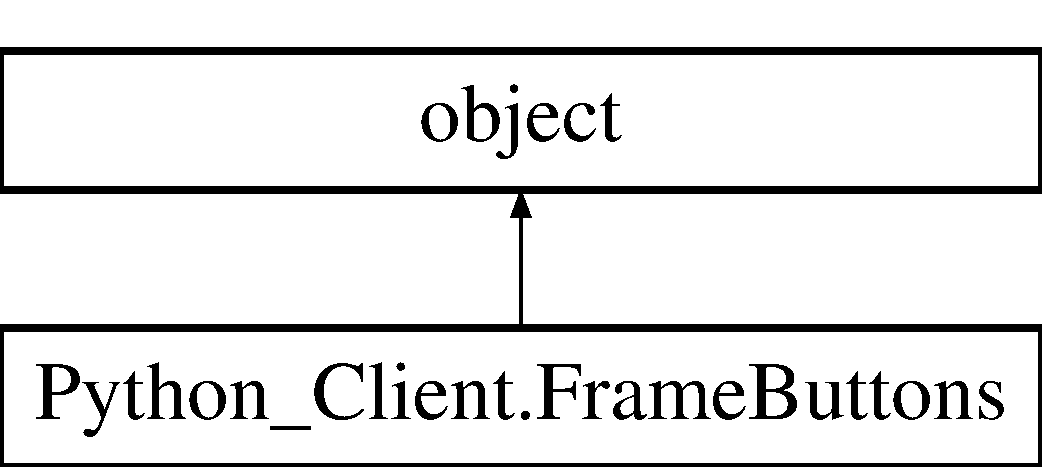
\includegraphics[height=2.000000cm]{class_python___client_1_1_frame_buttons}
\end{center}
\end{figure}
\subsection*{Public Member Functions}
\begin{DoxyCompactItemize}
\item 
def \mbox{\hyperlink{class_python___client_1_1_frame_buttons_a903927dea8f58c84d0a28ce980d1914a}{\+\_\+\+\_\+init\+\_\+\+\_\+}} (self, frame, name, nr)
\begin{DoxyCompactList}\small\item\em The default constructor. \end{DoxyCompactList}\item 
def \mbox{\hyperlink{class_python___client_1_1_frame_buttons_aeb5a8761dfb5bf6c2c1bd96ffee5f8fe}{create\+\_\+button}} (self)
\begin{DoxyCompactList}\small\item\em creates the button \end{DoxyCompactList}\item 
def \mbox{\hyperlink{class_python___client_1_1_frame_buttons_abeb6a6d56e4f66ae470b10ac5c849ebb}{frame\+\_\+switch}} (self)
\begin{DoxyCompactList}\small\item\em switches frames acording to the pressed button \end{DoxyCompactList}\end{DoxyCompactItemize}
\subsection*{Public Attributes}
\begin{DoxyCompactItemize}
\item 
\mbox{\Hypertarget{class_python___client_1_1_frame_buttons_a05df5a686b0be0cfe0f3fec43dd1610b}\label{class_python___client_1_1_frame_buttons_a05df5a686b0be0cfe0f3fec43dd1610b}} 
{\bfseries frame}
\item 
\mbox{\Hypertarget{class_python___client_1_1_frame_buttons_aebc39e17fde8bc095a65cf5395ae7da3}\label{class_python___client_1_1_frame_buttons_aebc39e17fde8bc095a65cf5395ae7da3}} 
{\bfseries name}
\item 
\mbox{\Hypertarget{class_python___client_1_1_frame_buttons_a8578c244ff1c429cf3ee508993ae9ac8}\label{class_python___client_1_1_frame_buttons_a8578c244ff1c429cf3ee508993ae9ac8}} 
{\bfseries nr}
\item 
\mbox{\Hypertarget{class_python___client_1_1_frame_buttons_a46d4384e43fbd5c22512088344f90a5f}\label{class_python___client_1_1_frame_buttons_a46d4384e43fbd5c22512088344f90a5f}} 
{\bfseries button}
\end{DoxyCompactItemize}


\subsection{Detailed Description}
This class handles the frame switch buttons. 

The class \mbox{\hyperlink{class_python___client_1_1_frame_buttons}{Frame\+Buttons}} creates and handles the frame switch buttons 

\subsection{Constructor \& Destructor Documentation}
\mbox{\Hypertarget{class_python___client_1_1_frame_buttons_a903927dea8f58c84d0a28ce980d1914a}\label{class_python___client_1_1_frame_buttons_a903927dea8f58c84d0a28ce980d1914a}} 
\index{Python\+\_\+\+Client\+::\+Frame\+Buttons@{Python\+\_\+\+Client\+::\+Frame\+Buttons}!\+\_\+\+\_\+init\+\_\+\+\_\+@{\+\_\+\+\_\+init\+\_\+\+\_\+}}
\index{\+\_\+\+\_\+init\+\_\+\+\_\+@{\+\_\+\+\_\+init\+\_\+\+\_\+}!Python\+\_\+\+Client\+::\+Frame\+Buttons@{Python\+\_\+\+Client\+::\+Frame\+Buttons}}
\subsubsection{\texorpdfstring{\+\_\+\+\_\+init\+\_\+\+\_\+()}{\_\_init\_\_()}}
{\footnotesize\ttfamily def Python\+\_\+\+Client.\+Frame\+Buttons.\+\_\+\+\_\+init\+\_\+\+\_\+ (\begin{DoxyParamCaption}\item[{}]{self,  }\item[{}]{frame,  }\item[{}]{name,  }\item[{}]{nr }\end{DoxyParamCaption})}



The default constructor. 

here the informations for the buttons will be saved in the Class Object


\begin{DoxyParams}{Parameters}
{\em frame} & contains the parent frame / window of the button \\
\hline
{\em name} & contains the text/name of the button \\
\hline
{\em nr} & contains the number/id of the button (for the frame\+\_\+switch method) \\
\hline
\end{DoxyParams}


\subsection{Member Function Documentation}
\mbox{\Hypertarget{class_python___client_1_1_frame_buttons_aeb5a8761dfb5bf6c2c1bd96ffee5f8fe}\label{class_python___client_1_1_frame_buttons_aeb5a8761dfb5bf6c2c1bd96ffee5f8fe}} 
\index{Python\+\_\+\+Client\+::\+Frame\+Buttons@{Python\+\_\+\+Client\+::\+Frame\+Buttons}!create\+\_\+button@{create\+\_\+button}}
\index{create\+\_\+button@{create\+\_\+button}!Python\+\_\+\+Client\+::\+Frame\+Buttons@{Python\+\_\+\+Client\+::\+Frame\+Buttons}}
\subsubsection{\texorpdfstring{create\+\_\+button()}{create\_button()}}
{\footnotesize\ttfamily def Python\+\_\+\+Client.\+Frame\+Buttons.\+create\+\_\+button (\begin{DoxyParamCaption}\item[{}]{self }\end{DoxyParamCaption})}



creates the button 

this method creates the button witch the according colors and command and places them with the .grid method from tkinter \mbox{\Hypertarget{class_python___client_1_1_frame_buttons_abeb6a6d56e4f66ae470b10ac5c849ebb}\label{class_python___client_1_1_frame_buttons_abeb6a6d56e4f66ae470b10ac5c849ebb}} 
\index{Python\+\_\+\+Client\+::\+Frame\+Buttons@{Python\+\_\+\+Client\+::\+Frame\+Buttons}!frame\+\_\+switch@{frame\+\_\+switch}}
\index{frame\+\_\+switch@{frame\+\_\+switch}!Python\+\_\+\+Client\+::\+Frame\+Buttons@{Python\+\_\+\+Client\+::\+Frame\+Buttons}}
\subsubsection{\texorpdfstring{frame\+\_\+switch()}{frame\_switch()}}
{\footnotesize\ttfamily def Python\+\_\+\+Client.\+Frame\+Buttons.\+frame\+\_\+switch (\begin{DoxyParamCaption}\item[{}]{self }\end{DoxyParamCaption})}



switches frames acording to the pressed button 

this method is executed, when a frame switch button is pressed, so that the frames switch accordingly 

The documentation for this class was generated from the following file\+:\begin{DoxyCompactItemize}
\item 
Python\+\_\+\+Client.\+py\end{DoxyCompactItemize}

\hypertarget{class_python___client_1_1send_mail}{}\section{Python\+\_\+\+Client.\+send\+Mail Class Reference}
\label{class_python___client_1_1send_mail}\index{Python\+\_\+\+Client.\+send\+Mail@{Python\+\_\+\+Client.\+send\+Mail}}


class to send emails  


Inheritance diagram for Python\+\_\+\+Client.\+send\+Mail\+:\begin{figure}[H]
\begin{center}
\leavevmode
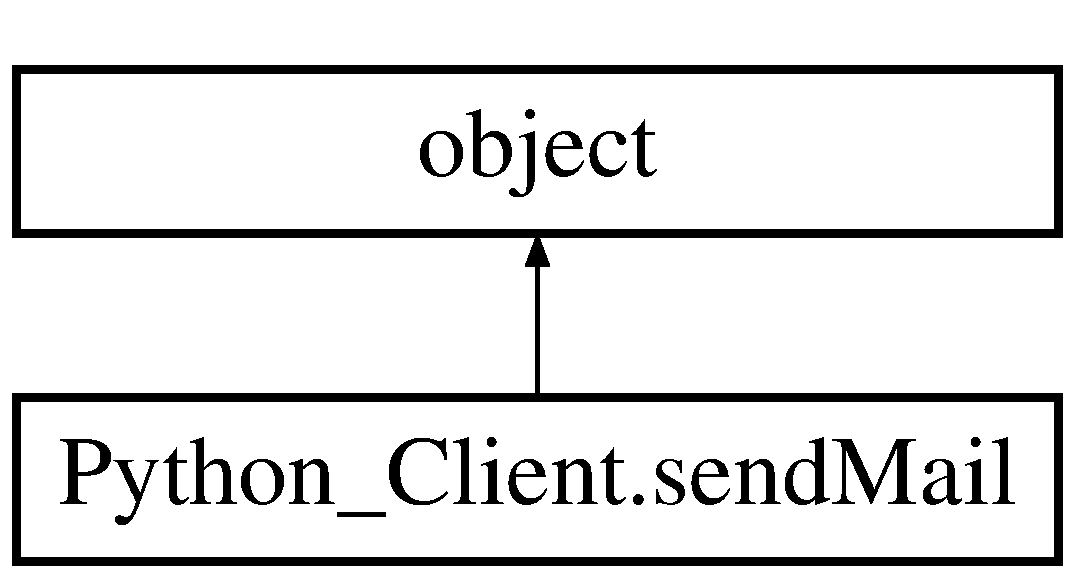
\includegraphics[height=2.000000cm]{class_python___client_1_1send_mail}
\end{center}
\end{figure}
\subsection*{Public Member Functions}
\begin{DoxyCompactItemize}
\item 
def \mbox{\hyperlink{class_python___client_1_1send_mail_abbe76ea5ec26636335cc40c07e1746c6}{\+\_\+\+\_\+init\+\_\+\+\_\+}} (self)
\begin{DoxyCompactList}\small\item\em The default constructor. \end{DoxyCompactList}\item 
def \mbox{\hyperlink{class_python___client_1_1send_mail_a5d245cd00e2df903015928d0902632d8}{sendmail}} (self, receiver, msg)
\begin{DoxyCompactList}\small\item\em method to send an E-\/\+Mail \end{DoxyCompactList}\item 
\mbox{\Hypertarget{class_python___client_1_1send_mail_a333f9ed9a6c5499d92955ebd8ddb0399}\label{class_python___client_1_1send_mail_a333f9ed9a6c5499d92955ebd8ddb0399}} 
def \mbox{\hyperlink{class_python___client_1_1send_mail_a333f9ed9a6c5499d92955ebd8ddb0399}{close}} (self)
\begin{DoxyCompactList}\small\item\em method to close the S\+M\+TP server connection \end{DoxyCompactList}\end{DoxyCompactItemize}
\subsection*{Public Attributes}
\begin{DoxyCompactItemize}
\item 
\mbox{\Hypertarget{class_python___client_1_1send_mail_a40f6fd6846557da60cf0c2e99847e550}\label{class_python___client_1_1send_mail_a40f6fd6846557da60cf0c2e99847e550}} 
{\bfseries server}
\item 
\mbox{\Hypertarget{class_python___client_1_1send_mail_a36ecd0c14687eec0c359e1d0a4abfd4b}\label{class_python___client_1_1send_mail_a36ecd0c14687eec0c359e1d0a4abfd4b}} 
{\bfseries receiver}
\item 
\mbox{\Hypertarget{class_python___client_1_1send_mail_a7b05c0042d54088efe3fb106fbcc821e}\label{class_python___client_1_1send_mail_a7b05c0042d54088efe3fb106fbcc821e}} 
{\bfseries msg}
\end{DoxyCompactItemize}


\subsection{Detailed Description}
class to send emails 

in this class an email can be send to an defined adress 

\subsection{Constructor \& Destructor Documentation}
\mbox{\Hypertarget{class_python___client_1_1send_mail_abbe76ea5ec26636335cc40c07e1746c6}\label{class_python___client_1_1send_mail_abbe76ea5ec26636335cc40c07e1746c6}} 
\index{Python\+\_\+\+Client\+::send\+Mail@{Python\+\_\+\+Client\+::send\+Mail}!\+\_\+\+\_\+init\+\_\+\+\_\+@{\+\_\+\+\_\+init\+\_\+\+\_\+}}
\index{\+\_\+\+\_\+init\+\_\+\+\_\+@{\+\_\+\+\_\+init\+\_\+\+\_\+}!Python\+\_\+\+Client\+::send\+Mail@{Python\+\_\+\+Client\+::send\+Mail}}
\subsubsection{\texorpdfstring{\+\_\+\+\_\+init\+\_\+\+\_\+()}{\_\_init\_\_()}}
{\footnotesize\ttfamily def Python\+\_\+\+Client.\+send\+Mail.\+\_\+\+\_\+init\+\_\+\+\_\+ (\begin{DoxyParamCaption}\item[{}]{self }\end{DoxyParamCaption})}



The default constructor. 

the Smtp server will be initialized in this constructor


\begin{DoxyParams}{Parameters}
{\em server} & the S\+M\+TP server connection (here gmail) \\
\hline
\end{DoxyParams}


\subsection{Member Function Documentation}
\mbox{\Hypertarget{class_python___client_1_1send_mail_a5d245cd00e2df903015928d0902632d8}\label{class_python___client_1_1send_mail_a5d245cd00e2df903015928d0902632d8}} 
\index{Python\+\_\+\+Client\+::send\+Mail@{Python\+\_\+\+Client\+::send\+Mail}!sendmail@{sendmail}}
\index{sendmail@{sendmail}!Python\+\_\+\+Client\+::send\+Mail@{Python\+\_\+\+Client\+::send\+Mail}}
\subsubsection{\texorpdfstring{sendmail()}{sendmail()}}
{\footnotesize\ttfamily def Python\+\_\+\+Client.\+send\+Mail.\+sendmail (\begin{DoxyParamCaption}\item[{}]{self,  }\item[{}]{receiver,  }\item[{}]{msg }\end{DoxyParamCaption})}



method to send an E-\/\+Mail 

here the the e-\/mail will be send wit a given message and receiver


\begin{DoxyParams}{Parameters}
{\em receiver} & e-\/mail adress to which the e-\/mail will be send \\
\hline
{\em msg} & the content of the e-\/mail \\
\hline
\end{DoxyParams}


The documentation for this class was generated from the following file\+:\begin{DoxyCompactItemize}
\item 
Python\+\_\+\+Client.\+py\end{DoxyCompactItemize}

\hypertarget{class_python___client_1_1_wifi_connect}{}\section{Python\+\_\+\+Client.\+Wifi\+Connect Class Reference}
\label{class_python___client_1_1_wifi_connect}\index{Python\+\_\+\+Client.\+Wifi\+Connect@{Python\+\_\+\+Client.\+Wifi\+Connect}}


a class for the Wifi connection  


Inheritance diagram for Python\+\_\+\+Client.\+Wifi\+Connect\+:\begin{figure}[H]
\begin{center}
\leavevmode
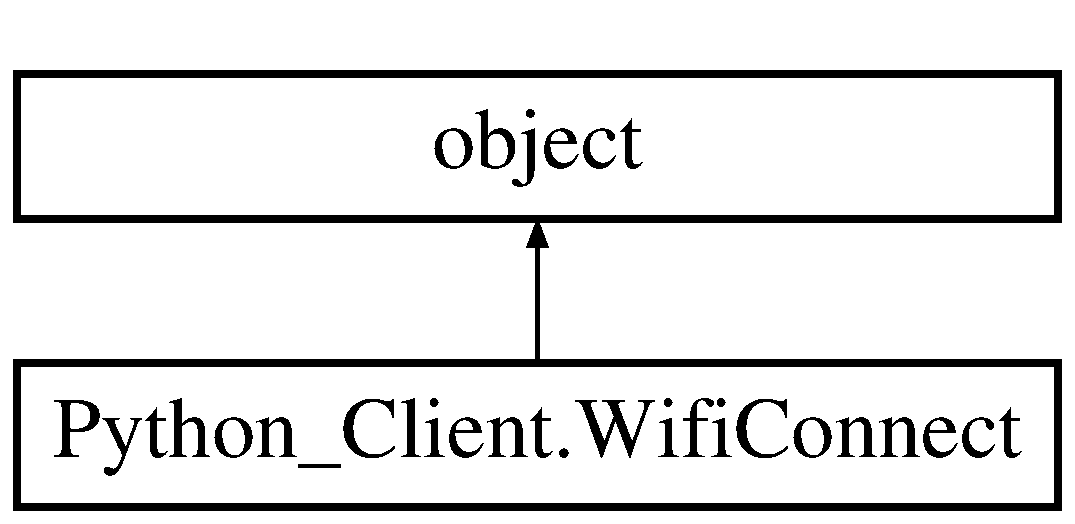
\includegraphics[height=2.000000cm]{class_python___client_1_1_wifi_connect}
\end{center}
\end{figure}
\subsection*{Public Member Functions}
\begin{DoxyCompactItemize}
\item 
def \mbox{\hyperlink{class_python___client_1_1_wifi_connect_a5abd335772d88bbc04fee603eed75852}{\+\_\+\+\_\+init\+\_\+\+\_\+}} (self, window, T\+C\+P\+\_\+\+IP, T\+C\+P\+\_\+\+P\+O\+RT, on\+\_\+receive)
\begin{DoxyCompactList}\small\item\em the default constructor \end{DoxyCompactList}\item 
def \mbox{\hyperlink{class_python___client_1_1_wifi_connect_ad5bac3310c58f99485738c056718a3ca}{send\+\_\+msg}} (self, message)
\begin{DoxyCompactList}\small\item\em Sends message to the arduino. \end{DoxyCompactList}\item 
def \mbox{\hyperlink{class_python___client_1_1_wifi_connect_ac05ef987e930e48c8c5bb8056c2ca68b}{close}} (self)
\begin{DoxyCompactList}\small\item\em close the connection \end{DoxyCompactList}\item 
def \mbox{\hyperlink{class_python___client_1_1_wifi_connect_a6eb0999228a1fc0e8f76d7aad443b6c5}{periodic\+\_\+socket\+\_\+check}} (self)
\begin{DoxyCompactList}\small\item\em checks for received message \end{DoxyCompactList}\end{DoxyCompactItemize}
\subsection*{Public Attributes}
\begin{DoxyCompactItemize}
\item 
\mbox{\Hypertarget{class_python___client_1_1_wifi_connect_a56ccc377926c457d236d91b299776574}\label{class_python___client_1_1_wifi_connect_a56ccc377926c457d236d91b299776574}} 
{\bfseries window}
\item 
\mbox{\Hypertarget{class_python___client_1_1_wifi_connect_a95b489d481322d5a7b320095dd13d563}\label{class_python___client_1_1_wifi_connect_a95b489d481322d5a7b320095dd13d563}} 
{\bfseries on\+\_\+receive}
\item 
\mbox{\Hypertarget{class_python___client_1_1_wifi_connect_a86da1a7e9cf31bd8085061341ab4e6b7}\label{class_python___client_1_1_wifi_connect_a86da1a7e9cf31bd8085061341ab4e6b7}} 
{\bfseries socket}
\item 
\mbox{\Hypertarget{class_python___client_1_1_wifi_connect_a70bd3f97800dff409d3773c07bdb98d6}\label{class_python___client_1_1_wifi_connect_a70bd3f97800dff409d3773c07bdb98d6}} 
\mbox{\hyperlink{class_python___client_1_1_wifi_connect_a70bd3f97800dff409d3773c07bdb98d6}{rd\+\_\+buff}}
\begin{DoxyCompactList}\small\item\em connect to the arduino \end{DoxyCompactList}\item 
\mbox{\Hypertarget{class_python___client_1_1_wifi_connect_aeb42d01979f3311563dbcc9a3d027b99}\label{class_python___client_1_1_wifi_connect_aeb42d01979f3311563dbcc9a3d027b99}} 
\mbox{\hyperlink{class_python___client_1_1_wifi_connect_aeb42d01979f3311563dbcc9a3d027b99}{after\+\_\+event}}
\begin{DoxyCompactList}\small\item\em if a message has been received, the message will be send to the on\+\_\+receive method \end{DoxyCompactList}\end{DoxyCompactItemize}


\subsection{Detailed Description}
a class for the Wifi connection 

This class handles the connection between the arduino and the python program and also contains the methods to send and receive messages through the wirelles connection 

\subsection{Constructor \& Destructor Documentation}
\mbox{\Hypertarget{class_python___client_1_1_wifi_connect_a5abd335772d88bbc04fee603eed75852}\label{class_python___client_1_1_wifi_connect_a5abd335772d88bbc04fee603eed75852}} 
\index{Python\+\_\+\+Client\+::\+Wifi\+Connect@{Python\+\_\+\+Client\+::\+Wifi\+Connect}!\+\_\+\+\_\+init\+\_\+\+\_\+@{\+\_\+\+\_\+init\+\_\+\+\_\+}}
\index{\+\_\+\+\_\+init\+\_\+\+\_\+@{\+\_\+\+\_\+init\+\_\+\+\_\+}!Python\+\_\+\+Client\+::\+Wifi\+Connect@{Python\+\_\+\+Client\+::\+Wifi\+Connect}}
\subsubsection{\texorpdfstring{\+\_\+\+\_\+init\+\_\+\+\_\+()}{\_\_init\_\_()}}
{\footnotesize\ttfamily def Python\+\_\+\+Client.\+Wifi\+Connect.\+\_\+\+\_\+init\+\_\+\+\_\+ (\begin{DoxyParamCaption}\item[{}]{self,  }\item[{}]{window,  }\item[{}]{T\+C\+P\+\_\+\+IP,  }\item[{}]{T\+C\+P\+\_\+\+P\+O\+RT,  }\item[{}]{on\+\_\+receive }\end{DoxyParamCaption})}



the default constructor 

This method handles the connection between the arduino and the python program as a client


\begin{DoxyParams}{Parameters}
{\em window} & The parent (root) window \\
\hline
{\em T\+C\+P\+\_\+\+IP} & Ip addres of the arduino \\
\hline
{\em T\+C\+P\+\_\+\+P\+O\+RT} & Port of the arduino \\
\hline
{\em on\+\_\+receive} & function to run when receiving a message from the arduino \\
\hline
{\em window} & parent window safed as local variable in the class \\
\hline
{\em on\+\_\+receive} & on\+\_\+receive function safed as local variable in the class \\
\hline
{\em socket} & safe the socket library as socket \\
\hline
\end{DoxyParams}


\subsection{Member Function Documentation}
\mbox{\Hypertarget{class_python___client_1_1_wifi_connect_ac05ef987e930e48c8c5bb8056c2ca68b}\label{class_python___client_1_1_wifi_connect_ac05ef987e930e48c8c5bb8056c2ca68b}} 
\index{Python\+\_\+\+Client\+::\+Wifi\+Connect@{Python\+\_\+\+Client\+::\+Wifi\+Connect}!close@{close}}
\index{close@{close}!Python\+\_\+\+Client\+::\+Wifi\+Connect@{Python\+\_\+\+Client\+::\+Wifi\+Connect}}
\subsubsection{\texorpdfstring{close()}{close()}}
{\footnotesize\ttfamily def Python\+\_\+\+Client.\+Wifi\+Connect.\+close (\begin{DoxyParamCaption}\item[{}]{self }\end{DoxyParamCaption})}



close the connection 

This method closes the connection between the arduino and the python program \mbox{\Hypertarget{class_python___client_1_1_wifi_connect_a6eb0999228a1fc0e8f76d7aad443b6c5}\label{class_python___client_1_1_wifi_connect_a6eb0999228a1fc0e8f76d7aad443b6c5}} 
\index{Python\+\_\+\+Client\+::\+Wifi\+Connect@{Python\+\_\+\+Client\+::\+Wifi\+Connect}!periodic\+\_\+socket\+\_\+check@{periodic\+\_\+socket\+\_\+check}}
\index{periodic\+\_\+socket\+\_\+check@{periodic\+\_\+socket\+\_\+check}!Python\+\_\+\+Client\+::\+Wifi\+Connect@{Python\+\_\+\+Client\+::\+Wifi\+Connect}}
\subsubsection{\texorpdfstring{periodic\+\_\+socket\+\_\+check()}{periodic\_socket\_check()}}
{\footnotesize\ttfamily def Python\+\_\+\+Client.\+Wifi\+Connect.\+periodic\+\_\+socket\+\_\+check (\begin{DoxyParamCaption}\item[{}]{self }\end{DoxyParamCaption})}



checks for received message 

This method checks, if a message from the arduino has been send to the python programm in a periodic frequence 
\begin{DoxyParams}{Parameters}
{\em line} & here the received message is saved \\
\hline
\end{DoxyParams}
\mbox{\Hypertarget{class_python___client_1_1_wifi_connect_ad5bac3310c58f99485738c056718a3ca}\label{class_python___client_1_1_wifi_connect_ad5bac3310c58f99485738c056718a3ca}} 
\index{Python\+\_\+\+Client\+::\+Wifi\+Connect@{Python\+\_\+\+Client\+::\+Wifi\+Connect}!send\+\_\+msg@{send\+\_\+msg}}
\index{send\+\_\+msg@{send\+\_\+msg}!Python\+\_\+\+Client\+::\+Wifi\+Connect@{Python\+\_\+\+Client\+::\+Wifi\+Connect}}
\subsubsection{\texorpdfstring{send\+\_\+msg()}{send\_msg()}}
{\footnotesize\ttfamily def Python\+\_\+\+Client.\+Wifi\+Connect.\+send\+\_\+msg (\begin{DoxyParamCaption}\item[{}]{self,  }\item[{}]{message }\end{DoxyParamCaption})}



Sends message to the arduino. 

This method sends a message to the E\+SP server (arduino)


\begin{DoxyParams}{Parameters}
{\em message} & contains the message to be send in bytes \\
\hline
\end{DoxyParams}


The documentation for this class was generated from the following file\+:\begin{DoxyCompactItemize}
\item 
Python\+\_\+\+Client.\+py\end{DoxyCompactItemize}

\hypertarget{class_python___client_1_1_window_function}{}\section{Python\+\_\+\+Client.\+Window\+Function Class Reference}
\label{class_python___client_1_1_window_function}\index{Python\+\_\+\+Client.\+Window\+Function@{Python\+\_\+\+Client.\+Window\+Function}}


The class to setup the main tkinter window.  


Inheritance diagram for Python\+\_\+\+Client.\+Window\+Function\+:\begin{figure}[H]
\begin{center}
\leavevmode
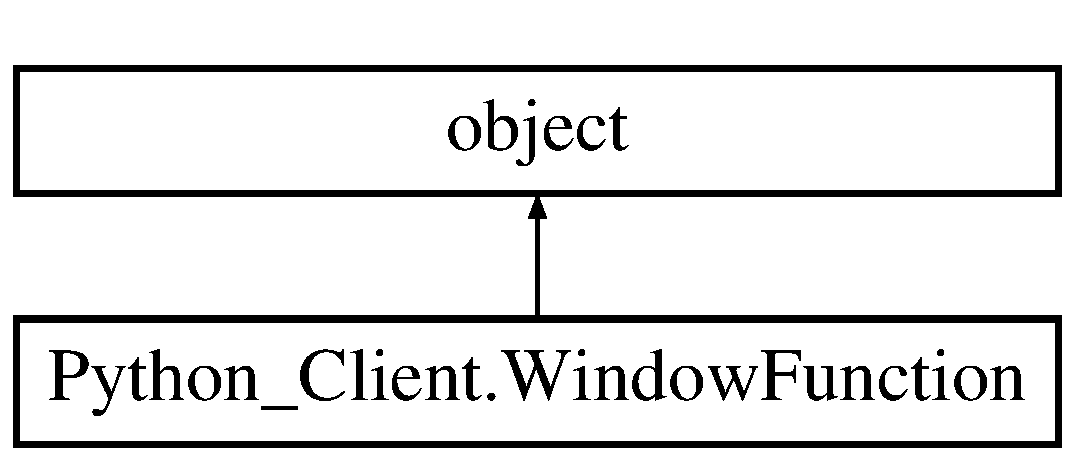
\includegraphics[height=2.000000cm]{class_python___client_1_1_window_function}
\end{center}
\end{figure}
\subsection*{Public Member Functions}
\begin{DoxyCompactItemize}
\item 
def \mbox{\hyperlink{class_python___client_1_1_window_function_a01d8492097a4aec1382b7d5611e539dd}{\+\_\+\+\_\+init\+\_\+\+\_\+}} (self)
\begin{DoxyCompactList}\small\item\em The default constructor. \end{DoxyCompactList}\item 
def \mbox{\hyperlink{class_python___client_1_1_window_function_aec21cc89e2085eb8d8adabf018ccd0eb}{on\+\_\+receive}} (self, line)
\begin{DoxyCompactList}\small\item\em handels the received commands from the Arduino \end{DoxyCompactList}\item 
def \mbox{\hyperlink{class_python___client_1_1_window_function_a668170ed5685df325812a3293eea68a9}{setup\+\_\+window}} (self)
\begin{DoxyCompactList}\small\item\em this method creates the window \end{DoxyCompactList}\item 
def \mbox{\hyperlink{class_python___client_1_1_window_function_a468af5948b986f639f15ae2f5a490afb}{window\+\_\+close}} (self)
\begin{DoxyCompactList}\small\item\em handler for Window close \end{DoxyCompactList}\item 
\mbox{\Hypertarget{class_python___client_1_1_window_function_a0ba0640860866ac24b0972c5e40dbe8a}\label{class_python___client_1_1_window_function_a0ba0640860866ac24b0972c5e40dbe8a}} 
def \mbox{\hyperlink{class_python___client_1_1_window_function_a0ba0640860866ac24b0972c5e40dbe8a}{run}} (self)
\begin{DoxyCompactList}\small\item\em runs the tkinter module to show the window \end{DoxyCompactList}\item 
def \mbox{\hyperlink{class_python___client_1_1_window_function_a0059612952a6abcd18c39d5c1ea6cb9b}{setup\+\_\+framebtn}} (self)
\begin{DoxyCompactList}\small\item\em sets the frame buttons on window top \end{DoxyCompactList}\item 
def \mbox{\hyperlink{class_python___client_1_1_window_function_a1387df5915e23ef0d92a3e816d3f128b}{setup\+\_\+frames}} (self)
\begin{DoxyCompactList}\small\item\em this method sets the frames for the main functions of the project \end{DoxyCompactList}\item 
def \mbox{\hyperlink{class_python___client_1_1_window_function_a48e25dc456e930042a87bbec5239c458}{forget\+\_\+frames}} (self)
\begin{DoxyCompactList}\small\item\em let all frames dissapear (pack\+\_\+forget) \end{DoxyCompactList}\item 
def \mbox{\hyperlink{class_python___client_1_1_window_function_aab4df36ab3b25e679b67f09cde9d256d}{setup\+\_\+rgbframe}} (self)
\begin{DoxyCompactList}\small\item\em setup the rgb-\/frame widgets \end{DoxyCompactList}\item 
def \mbox{\hyperlink{class_python___client_1_1_window_function_a625d8169e5b5f11c4dd7df8611ff1ad0}{setup\+\_\+alarmframe}} (self)
\begin{DoxyCompactList}\small\item\em setup the alarm-\/frame widgets \end{DoxyCompactList}\item 
def \mbox{\hyperlink{class_python___client_1_1_window_function_a7973ce53af104391d4be0af460577b94}{setup\+\_\+welcomeframe}} (self)
\begin{DoxyCompactList}\small\item\em setup the welcome-\/frame widgets \end{DoxyCompactList}\item 
def \mbox{\hyperlink{class_python___client_1_1_window_function_af8c2258f6fc091b3fa7b077306f45b67}{alarm\+\_\+handler}} (self)
\begin{DoxyCompactList}\small\item\em method for the alarm button \end{DoxyCompactList}\item 
def \mbox{\hyperlink{class_python___client_1_1_window_function_a065ec1b6535adc5009029b90060ed44e}{choose\+\_\+color}} (self)
\begin{DoxyCompactList}\small\item\em method for the color choose button \end{DoxyCompactList}\item 
def \mbox{\hyperlink{class_python___client_1_1_window_function_a9b35486b2d7a0320f38feb86d568ed87}{lights\+\_\+off}} (self)
\begin{DoxyCompactList}\small\item\em method for the lights off button \end{DoxyCompactList}\end{DoxyCompactItemize}
\subsection*{Public Attributes}
\begin{DoxyCompactItemize}
\item 
\mbox{\Hypertarget{class_python___client_1_1_window_function_a0c0fa884f1138b278547d54acda2195e}\label{class_python___client_1_1_window_function_a0c0fa884f1138b278547d54acda2195e}} 
{\bfseries rgb\+\_\+red}
\item 
\mbox{\Hypertarget{class_python___client_1_1_window_function_afcc08523599fd4982099898ab3dc9399}\label{class_python___client_1_1_window_function_afcc08523599fd4982099898ab3dc9399}} 
{\bfseries rgb\+\_\+green}
\item 
\mbox{\Hypertarget{class_python___client_1_1_window_function_ac0b99ab6367531384ca989c738822974}\label{class_python___client_1_1_window_function_ac0b99ab6367531384ca989c738822974}} 
{\bfseries rgb\+\_\+blue}
\item 
\mbox{\Hypertarget{class_python___client_1_1_window_function_a8f6145a8a6176a5e75a7c050f0bdddad}\label{class_python___client_1_1_window_function_a8f6145a8a6176a5e75a7c050f0bdddad}} 
{\bfseries arduino}
\item 
\mbox{\Hypertarget{class_python___client_1_1_window_function_a414446a30687cc0039ce4493cb78ee8e}\label{class_python___client_1_1_window_function_a414446a30687cc0039ce4493cb78ee8e}} 
{\bfseries mailer}
\item 
\mbox{\Hypertarget{class_python___client_1_1_window_function_a9e10e8f492221b5fe234d944a9f2950d}\label{class_python___client_1_1_window_function_a9e10e8f492221b5fe234d944a9f2950d}} 
{\bfseries alarm\+\_\+status}
\item 
\mbox{\Hypertarget{class_python___client_1_1_window_function_a5b38a27683f302e4c928a4ce4381dc31}\label{class_python___client_1_1_window_function_a5b38a27683f302e4c928a4ce4381dc31}} 
{\bfseries window}
\item 
\mbox{\Hypertarget{class_python___client_1_1_window_function_a715bd4baaebf3bb52d8a117c28b40f24}\label{class_python___client_1_1_window_function_a715bd4baaebf3bb52d8a117c28b40f24}} 
{\bfseries frame}
\item 
\mbox{\Hypertarget{class_python___client_1_1_window_function_a17882e1223a151445da660bcfcb982ed}\label{class_python___client_1_1_window_function_a17882e1223a151445da660bcfcb982ed}} 
{\bfseries btn1}
\item 
\mbox{\Hypertarget{class_python___client_1_1_window_function_a3c1edccd45036585178bc18774680174}\label{class_python___client_1_1_window_function_a3c1edccd45036585178bc18774680174}} 
{\bfseries btn2}
\item 
\mbox{\Hypertarget{class_python___client_1_1_window_function_a2766dc911f9a24a6df890e4330ff5bd4}\label{class_python___client_1_1_window_function_a2766dc911f9a24a6df890e4330ff5bd4}} 
{\bfseries btn3}
\item 
\mbox{\Hypertarget{class_python___client_1_1_window_function_a8710e5c5a79b0253a35c4b769820e0b6}\label{class_python___client_1_1_window_function_a8710e5c5a79b0253a35c4b769820e0b6}} 
{\bfseries frame\+\_\+rgb}
\item 
\mbox{\Hypertarget{class_python___client_1_1_window_function_a44312387ca730d29b212ae01b0dc14cf}\label{class_python___client_1_1_window_function_a44312387ca730d29b212ae01b0dc14cf}} 
{\bfseries frame\+\_\+alarm}
\item 
\mbox{\Hypertarget{class_python___client_1_1_window_function_a951521d7d8d89b6ae737ab58db308fbd}\label{class_python___client_1_1_window_function_a951521d7d8d89b6ae737ab58db308fbd}} 
{\bfseries frame\+\_\+welcome}
\item 
\mbox{\Hypertarget{class_python___client_1_1_window_function_a16c3bf07132e4c655edd3b0303c4b9f2}\label{class_python___client_1_1_window_function_a16c3bf07132e4c655edd3b0303c4b9f2}} 
{\bfseries rgb\+\_\+title}
\item 
\mbox{\Hypertarget{class_python___client_1_1_window_function_a6e586e0731c26d28e151b7e23ee16499}\label{class_python___client_1_1_window_function_a6e586e0731c26d28e151b7e23ee16499}} 
{\bfseries color\+\_\+btn}
\item 
\mbox{\Hypertarget{class_python___client_1_1_window_function_a10734c7562a3b05d9b5541d447ab7d1f}\label{class_python___client_1_1_window_function_a10734c7562a3b05d9b5541d447ab7d1f}} 
{\bfseries rgb\+\_\+text}
\item 
\mbox{\Hypertarget{class_python___client_1_1_window_function_a9acfd7eb548138b32770d9b934b24d26}\label{class_python___client_1_1_window_function_a9acfd7eb548138b32770d9b934b24d26}} 
{\bfseries rgb\+\_\+description}
\item 
\mbox{\Hypertarget{class_python___client_1_1_window_function_a77ec36b5a5476f3d753db3b634d84950}\label{class_python___client_1_1_window_function_a77ec36b5a5476f3d753db3b634d84950}} 
{\bfseries rgb\+\_\+off\+\_\+btn}
\item 
\mbox{\Hypertarget{class_python___client_1_1_window_function_af482aee42f2b5bb723abbf4159a62e54}\label{class_python___client_1_1_window_function_af482aee42f2b5bb723abbf4159a62e54}} 
{\bfseries alarm\+\_\+title}
\item 
\mbox{\Hypertarget{class_python___client_1_1_window_function_ab43675dcd6b8697f5008c33f04fe44ca}\label{class_python___client_1_1_window_function_ab43675dcd6b8697f5008c33f04fe44ca}} 
{\bfseries alarm\+\_\+text}
\item 
\mbox{\Hypertarget{class_python___client_1_1_window_function_ac175ad2d731007f3714e4ff576afef6b}\label{class_python___client_1_1_window_function_ac175ad2d731007f3714e4ff576afef6b}} 
{\bfseries alarm\+\_\+description}
\item 
\mbox{\Hypertarget{class_python___client_1_1_window_function_a9c21f0b16d75b7c5077c77c4b2748013}\label{class_python___client_1_1_window_function_a9c21f0b16d75b7c5077c77c4b2748013}} 
{\bfseries alarm\+\_\+btn}
\item 
\mbox{\Hypertarget{class_python___client_1_1_window_function_a7b49e41bd8b8b3c8d4fbb67cfe1a0a41}\label{class_python___client_1_1_window_function_a7b49e41bd8b8b3c8d4fbb67cfe1a0a41}} 
{\bfseries welcome\+\_\+title}
\item 
\mbox{\Hypertarget{class_python___client_1_1_window_function_ae1eeba358d5e6c658eed7b7fbe678096}\label{class_python___client_1_1_window_function_ae1eeba358d5e6c658eed7b7fbe678096}} 
{\bfseries welcome\+\_\+text}
\item 
\mbox{\Hypertarget{class_python___client_1_1_window_function_ab1833e34efe0af6551de1de06a7ee2a9}\label{class_python___client_1_1_window_function_ab1833e34efe0af6551de1de06a7ee2a9}} 
{\bfseries welcome\+\_\+description}
\item 
\mbox{\hyperlink{class_python___client_1_1_window_function_a6c0768916064d607a4d39441863eabe2}{rgb}}
\begin{DoxyCompactList}\small\item\em the colorchooser.\+askcolor gives the rgb values as an two dimensional array e.\+g. \end{DoxyCompactList}\end{DoxyCompactItemize}


\subsection{Detailed Description}
The class to setup the main tkinter window. 

in this class the main window will created and the contend setup is executed 

\subsection{Constructor \& Destructor Documentation}
\mbox{\Hypertarget{class_python___client_1_1_window_function_a01d8492097a4aec1382b7d5611e539dd}\label{class_python___client_1_1_window_function_a01d8492097a4aec1382b7d5611e539dd}} 
\index{Python\+\_\+\+Client\+::\+Window\+Function@{Python\+\_\+\+Client\+::\+Window\+Function}!\+\_\+\+\_\+init\+\_\+\+\_\+@{\+\_\+\+\_\+init\+\_\+\+\_\+}}
\index{\+\_\+\+\_\+init\+\_\+\+\_\+@{\+\_\+\+\_\+init\+\_\+\+\_\+}!Python\+\_\+\+Client\+::\+Window\+Function@{Python\+\_\+\+Client\+::\+Window\+Function}}
\subsubsection{\texorpdfstring{\+\_\+\+\_\+init\+\_\+\+\_\+()}{\_\_init\_\_()}}
{\footnotesize\ttfamily def Python\+\_\+\+Client.\+Window\+Function.\+\_\+\+\_\+init\+\_\+\+\_\+ (\begin{DoxyParamCaption}\item[{}]{self }\end{DoxyParamCaption})}



The default constructor. 

The arduino and Email server connection will be initialized and all window setup methods will be executed


\begin{DoxyParams}{Parameters}
{\em rgb\+\_\+red} & red value for the rgb light \\
\hline
{\em rgb\+\_\+green} & green value for the rgb light \\
\hline
{\em rgb\+\_\+blue} & blue value for the rgb light \\
\hline
{\em arduino} & the Wifi\+Connection object \\
\hline
{\em mailer} & the \mbox{\hyperlink{class_python___client_1_1send_mail}{send\+Mail}} object \\
\hline
{\em host} & the IP address for the wifi connection \\
\hline
{\em port} & the port for the wifi connection \\
\hline
\end{DoxyParams}


\subsection{Member Function Documentation}
\mbox{\Hypertarget{class_python___client_1_1_window_function_af8c2258f6fc091b3fa7b077306f45b67}\label{class_python___client_1_1_window_function_af8c2258f6fc091b3fa7b077306f45b67}} 
\index{Python\+\_\+\+Client\+::\+Window\+Function@{Python\+\_\+\+Client\+::\+Window\+Function}!alarm\+\_\+handler@{alarm\+\_\+handler}}
\index{alarm\+\_\+handler@{alarm\+\_\+handler}!Python\+\_\+\+Client\+::\+Window\+Function@{Python\+\_\+\+Client\+::\+Window\+Function}}
\subsubsection{\texorpdfstring{alarm\+\_\+handler()}{alarm\_handler()}}
{\footnotesize\ttfamily def Python\+\_\+\+Client.\+Window\+Function.\+alarm\+\_\+handler (\begin{DoxyParamCaption}\item[{}]{self }\end{DoxyParamCaption})}



method for the alarm button 

this method will be executed, when the alarm button is pressed

the method will send messages to the arduino acordingly to the alarmstatus and also change the alarm button configuration. at the start of the message to the arduino there is alarm written, so that the arduino will know for what the message will be


\begin{DoxyParams}{Parameters}
{\em alarm\+\_\+status} & status of the alarm (0 = alarm off ; 1 = alarm active ; 2 = alarm triggered) \\
\hline
\end{DoxyParams}
\mbox{\Hypertarget{class_python___client_1_1_window_function_a065ec1b6535adc5009029b90060ed44e}\label{class_python___client_1_1_window_function_a065ec1b6535adc5009029b90060ed44e}} 
\index{Python\+\_\+\+Client\+::\+Window\+Function@{Python\+\_\+\+Client\+::\+Window\+Function}!choose\+\_\+color@{choose\+\_\+color}}
\index{choose\+\_\+color@{choose\+\_\+color}!Python\+\_\+\+Client\+::\+Window\+Function@{Python\+\_\+\+Client\+::\+Window\+Function}}
\subsubsection{\texorpdfstring{choose\+\_\+color()}{choose\_color()}}
{\footnotesize\ttfamily def Python\+\_\+\+Client.\+Window\+Function.\+choose\+\_\+color (\begin{DoxyParamCaption}\item[{}]{self }\end{DoxyParamCaption})}



method for the color choose button 

this method will be executed, when the color\+\_\+btn is pressed

this method asks for a color and saves it in the rgb variables, sends them to the arduino and changes the color of the button to the choosen color. at the start of the message there is rgb written, so that the arduino will know for what the message will be


\begin{DoxyParams}{Parameters}
{\em rgb} & \\
\hline
\end{DoxyParams}
\mbox{\Hypertarget{class_python___client_1_1_window_function_a48e25dc456e930042a87bbec5239c458}\label{class_python___client_1_1_window_function_a48e25dc456e930042a87bbec5239c458}} 
\index{Python\+\_\+\+Client\+::\+Window\+Function@{Python\+\_\+\+Client\+::\+Window\+Function}!forget\+\_\+frames@{forget\+\_\+frames}}
\index{forget\+\_\+frames@{forget\+\_\+frames}!Python\+\_\+\+Client\+::\+Window\+Function@{Python\+\_\+\+Client\+::\+Window\+Function}}
\subsubsection{\texorpdfstring{forget\+\_\+frames()}{forget\_frames()}}
{\footnotesize\ttfamily def Python\+\_\+\+Client.\+Window\+Function.\+forget\+\_\+frames (\begin{DoxyParamCaption}\item[{}]{self }\end{DoxyParamCaption})}



let all frames dissapear (pack\+\_\+forget) 

here all main frames will be unpacked, so they are not visible and the frame-\/switch-\/buttons color will be set to default

this method will be used in the \mbox{\hyperlink{class_python___client_1_1_frame_buttons}{Frame\+Buttons}} class for the frame\+\_\+switch method \mbox{\Hypertarget{class_python___client_1_1_window_function_a9b35486b2d7a0320f38feb86d568ed87}\label{class_python___client_1_1_window_function_a9b35486b2d7a0320f38feb86d568ed87}} 
\index{Python\+\_\+\+Client\+::\+Window\+Function@{Python\+\_\+\+Client\+::\+Window\+Function}!lights\+\_\+off@{lights\+\_\+off}}
\index{lights\+\_\+off@{lights\+\_\+off}!Python\+\_\+\+Client\+::\+Window\+Function@{Python\+\_\+\+Client\+::\+Window\+Function}}
\subsubsection{\texorpdfstring{lights\+\_\+off()}{lights\_off()}}
{\footnotesize\ttfamily def Python\+\_\+\+Client.\+Window\+Function.\+lights\+\_\+off (\begin{DoxyParamCaption}\item[{}]{self }\end{DoxyParamCaption})}



method for the lights off button 

this method will be executed, when the rgb\+\_\+off\+\_\+btn is pressed

this method sets the rgb variables to zero and sends these values to the arduino like in \mbox{\hyperlink{class_python___client_1_1_window_function_a065ec1b6535adc5009029b90060ed44e}{choose\+\_\+color()}} method \mbox{\Hypertarget{class_python___client_1_1_window_function_aec21cc89e2085eb8d8adabf018ccd0eb}\label{class_python___client_1_1_window_function_aec21cc89e2085eb8d8adabf018ccd0eb}} 
\index{Python\+\_\+\+Client\+::\+Window\+Function@{Python\+\_\+\+Client\+::\+Window\+Function}!on\+\_\+receive@{on\+\_\+receive}}
\index{on\+\_\+receive@{on\+\_\+receive}!Python\+\_\+\+Client\+::\+Window\+Function@{Python\+\_\+\+Client\+::\+Window\+Function}}
\subsubsection{\texorpdfstring{on\+\_\+receive()}{on\_receive()}}
{\footnotesize\ttfamily def Python\+\_\+\+Client.\+Window\+Function.\+on\+\_\+receive (\begin{DoxyParamCaption}\item[{}]{self,  }\item[{}]{line }\end{DoxyParamCaption})}



handels the received commands from the Arduino 

receives the the message from the arduino

when the message is \char`\"{}alarm\char`\"{} the rgb light will turn red, the button will be adjusted and the alarm status will turn to 2


\begin{DoxyParams}{Parameters}
{\em alarm\+\_\+status} & status of the alarm (0 = alarm off ; 1 = alarm active ; 2 = alarm triggered) \\
\hline
\end{DoxyParams}
\mbox{\Hypertarget{class_python___client_1_1_window_function_a625d8169e5b5f11c4dd7df8611ff1ad0}\label{class_python___client_1_1_window_function_a625d8169e5b5f11c4dd7df8611ff1ad0}} 
\index{Python\+\_\+\+Client\+::\+Window\+Function@{Python\+\_\+\+Client\+::\+Window\+Function}!setup\+\_\+alarmframe@{setup\+\_\+alarmframe}}
\index{setup\+\_\+alarmframe@{setup\+\_\+alarmframe}!Python\+\_\+\+Client\+::\+Window\+Function@{Python\+\_\+\+Client\+::\+Window\+Function}}
\subsubsection{\texorpdfstring{setup\+\_\+alarmframe()}{setup\_alarmframe()}}
{\footnotesize\ttfamily def Python\+\_\+\+Client.\+Window\+Function.\+setup\+\_\+alarmframe (\begin{DoxyParamCaption}\item[{}]{self }\end{DoxyParamCaption})}



setup the alarm-\/frame widgets 

in this method the contend of the alarm\+\_\+frame will be created and placed


\begin{DoxyParams}{Parameters}
{\em alarm\+\_\+title} & the label object for the title of the frame \\
\hline
{\em alarm\+\_\+text} & the description text \\
\hline
{\em alarm\+\_\+description} & the description label object with the description text as content \\
\hline
{\em alarm\+\_\+btn} & the button for the alarm control \\
\hline
\end{DoxyParams}
\mbox{\Hypertarget{class_python___client_1_1_window_function_a0059612952a6abcd18c39d5c1ea6cb9b}\label{class_python___client_1_1_window_function_a0059612952a6abcd18c39d5c1ea6cb9b}} 
\index{Python\+\_\+\+Client\+::\+Window\+Function@{Python\+\_\+\+Client\+::\+Window\+Function}!setup\+\_\+framebtn@{setup\+\_\+framebtn}}
\index{setup\+\_\+framebtn@{setup\+\_\+framebtn}!Python\+\_\+\+Client\+::\+Window\+Function@{Python\+\_\+\+Client\+::\+Window\+Function}}
\subsubsection{\texorpdfstring{setup\+\_\+framebtn()}{setup\_framebtn()}}
{\footnotesize\ttfamily def Python\+\_\+\+Client.\+Window\+Function.\+setup\+\_\+framebtn (\begin{DoxyParamCaption}\item[{}]{self }\end{DoxyParamCaption})}



sets the frame buttons on window top 

the frame-\/switch-\/button frame will created and right after the frame-\/switch-\/buttons


\begin{DoxyParams}{Parameters}
{\em frame} & the parent frame for the window switch buttons \\
\hline
{\em btn1} & first frame-\/switch-\/button \char`\"{}\+L\+I\+G\+H\+T\char`\"{} \\
\hline
{\em btn2} & second frame-\/switch-\/button \char`\"{}\+A\+L\+A\+R\+M\char`\"{} \\
\hline
{\em btn3} & third frame-\/switch-\/button \char`\"{}\+W\+E\+L\+C\+O\+M\+E\char`\"{} \\
\hline
\end{DoxyParams}
\mbox{\Hypertarget{class_python___client_1_1_window_function_a1387df5915e23ef0d92a3e816d3f128b}\label{class_python___client_1_1_window_function_a1387df5915e23ef0d92a3e816d3f128b}} 
\index{Python\+\_\+\+Client\+::\+Window\+Function@{Python\+\_\+\+Client\+::\+Window\+Function}!setup\+\_\+frames@{setup\+\_\+frames}}
\index{setup\+\_\+frames@{setup\+\_\+frames}!Python\+\_\+\+Client\+::\+Window\+Function@{Python\+\_\+\+Client\+::\+Window\+Function}}
\subsubsection{\texorpdfstring{setup\+\_\+frames()}{setup\_frames()}}
{\footnotesize\ttfamily def Python\+\_\+\+Client.\+Window\+Function.\+setup\+\_\+frames (\begin{DoxyParamCaption}\item[{}]{self }\end{DoxyParamCaption})}



this method sets the frames for the main functions of the project 

the main frames will be created and the on program start opened frame will be packed, so it is visible


\begin{DoxyParams}{Parameters}
{\em frame\+\_\+rgb} & \\
\hline
{\em frame\+\_\+alarm} & \\
\hline
{\em frame\+\_\+welcome} & \\
\hline
\end{DoxyParams}
\mbox{\Hypertarget{class_python___client_1_1_window_function_aab4df36ab3b25e679b67f09cde9d256d}\label{class_python___client_1_1_window_function_aab4df36ab3b25e679b67f09cde9d256d}} 
\index{Python\+\_\+\+Client\+::\+Window\+Function@{Python\+\_\+\+Client\+::\+Window\+Function}!setup\+\_\+rgbframe@{setup\+\_\+rgbframe}}
\index{setup\+\_\+rgbframe@{setup\+\_\+rgbframe}!Python\+\_\+\+Client\+::\+Window\+Function@{Python\+\_\+\+Client\+::\+Window\+Function}}
\subsubsection{\texorpdfstring{setup\+\_\+rgbframe()}{setup\_rgbframe()}}
{\footnotesize\ttfamily def Python\+\_\+\+Client.\+Window\+Function.\+setup\+\_\+rgbframe (\begin{DoxyParamCaption}\item[{}]{self }\end{DoxyParamCaption})}



setup the rgb-\/frame widgets 

in this method the contend of the rgb\+\_\+frame will be created and placed


\begin{DoxyParams}{Parameters}
{\em rgb\+\_\+title} & the label object for the title of the frame ~\newline
\\
\hline
{\em color\+\_\+btn} & the button for the color selection \\
\hline
{\em rgb\+\_\+text} & the description text \\
\hline
{\em rgb\+\_\+description} & the description label object with the description text as content \\
\hline
{\em rgb\+\_\+off\+\_\+btn} & button to set the rgb values to zero (turn rgb led off) \\
\hline
\end{DoxyParams}
\mbox{\Hypertarget{class_python___client_1_1_window_function_a7973ce53af104391d4be0af460577b94}\label{class_python___client_1_1_window_function_a7973ce53af104391d4be0af460577b94}} 
\index{Python\+\_\+\+Client\+::\+Window\+Function@{Python\+\_\+\+Client\+::\+Window\+Function}!setup\+\_\+welcomeframe@{setup\+\_\+welcomeframe}}
\index{setup\+\_\+welcomeframe@{setup\+\_\+welcomeframe}!Python\+\_\+\+Client\+::\+Window\+Function@{Python\+\_\+\+Client\+::\+Window\+Function}}
\subsubsection{\texorpdfstring{setup\+\_\+welcomeframe()}{setup\_welcomeframe()}}
{\footnotesize\ttfamily def Python\+\_\+\+Client.\+Window\+Function.\+setup\+\_\+welcomeframe (\begin{DoxyParamCaption}\item[{}]{self }\end{DoxyParamCaption})}



setup the welcome-\/frame widgets 

in this method the contend of the welcome\+\_\+frame will be created and placed


\begin{DoxyParams}{Parameters}
{\em welcome\+\_\+title} & the label object for the title of the frame \\
\hline
{\em welcome\+\_\+text} & the description text \\
\hline
{\em welcome\+\_\+description} & the description label object with the description text as content \\
\hline
\end{DoxyParams}
\mbox{\Hypertarget{class_python___client_1_1_window_function_a668170ed5685df325812a3293eea68a9}\label{class_python___client_1_1_window_function_a668170ed5685df325812a3293eea68a9}} 
\index{Python\+\_\+\+Client\+::\+Window\+Function@{Python\+\_\+\+Client\+::\+Window\+Function}!setup\+\_\+window@{setup\+\_\+window}}
\index{setup\+\_\+window@{setup\+\_\+window}!Python\+\_\+\+Client\+::\+Window\+Function@{Python\+\_\+\+Client\+::\+Window\+Function}}
\subsubsection{\texorpdfstring{setup\+\_\+window()}{setup\_window()}}
{\footnotesize\ttfamily def Python\+\_\+\+Client.\+Window\+Function.\+setup\+\_\+window (\begin{DoxyParamCaption}\item[{}]{self }\end{DoxyParamCaption})}



this method creates the window 

this method creates the window with the a given title, geometry and an window delete protocol (method window\+\_\+close) \mbox{\Hypertarget{class_python___client_1_1_window_function_a468af5948b986f639f15ae2f5a490afb}\label{class_python___client_1_1_window_function_a468af5948b986f639f15ae2f5a490afb}} 
\index{Python\+\_\+\+Client\+::\+Window\+Function@{Python\+\_\+\+Client\+::\+Window\+Function}!window\+\_\+close@{window\+\_\+close}}
\index{window\+\_\+close@{window\+\_\+close}!Python\+\_\+\+Client\+::\+Window\+Function@{Python\+\_\+\+Client\+::\+Window\+Function}}
\subsubsection{\texorpdfstring{window\+\_\+close()}{window\_close()}}
{\footnotesize\ttfamily def Python\+\_\+\+Client.\+Window\+Function.\+window\+\_\+close (\begin{DoxyParamCaption}\item[{}]{self }\end{DoxyParamCaption})}



handler for Window close 

by closing the window first the arduino and S\+M\+TP connection will be closed 

\subsection{Member Data Documentation}
\mbox{\Hypertarget{class_python___client_1_1_window_function_a6c0768916064d607a4d39441863eabe2}\label{class_python___client_1_1_window_function_a6c0768916064d607a4d39441863eabe2}} 
\index{Python\+\_\+\+Client\+::\+Window\+Function@{Python\+\_\+\+Client\+::\+Window\+Function}!rgb@{rgb}}
\index{rgb@{rgb}!Python\+\_\+\+Client\+::\+Window\+Function@{Python\+\_\+\+Client\+::\+Window\+Function}}
\subsubsection{\texorpdfstring{rgb}{rgb}}
{\footnotesize\ttfamily Python\+\_\+\+Client.\+Window\+Function.\+rgb}



the colorchooser.\+askcolor gives the rgb values as an two dimensional array e.\+g. 

\mbox{[}(255, 255, 255),(\#\+F\+F\+F\+F\+FF)\mbox{]} 

The documentation for this class was generated from the following file\+:\begin{DoxyCompactItemize}
\item 
Python\+\_\+\+Client.\+py\end{DoxyCompactItemize}

%--- End generated contents ---

% Index
\backmatter
\newpage
\phantomsection
\clearemptydoublepage
\addcontentsline{toc}{chapter}{Index}
\printindex

\end{document}
